\documentclass[letterpaper,english,prl,reprint,longbibliography]{revtex4-1} %twocolumn,

%\usepackage[latin9]{inputenc}
\setcounter{secnumdepth}{3}
\usepackage{babel}
\usepackage{amsmath}
\usepackage{amssymb}
\usepackage{graphicx} 
\usepackage{epstopdf} %add for pdflatex, nut don't compile because of invisible character copied from .bbl file?
\usepackage[T1]{fontenc}
\usepackage[utf8x]{inputenc} 
\usepackage{esint}
%\usepackage[hyphens]{url}
\usepackage[unicode=true]{hyperref}
\usepackage[table]{xcolor}
%\loadpackage{url}
%\usepackage[unicode=true]{hyperref}
%\setcounter{biburllcpenalty}{7000}
%\setcounter{biburlucpenalty}{8000}
%\usepackage{breakurl}
%\hypersetup{breaklinks=true}
%\usepackage[hyperref,eprint=false]{biblatex}
\makeatletter

%%%%%%%%%%%%%%%%%%%%%%%%%%%%%% LyX specific LaTeX commands.
\pdfpageheight\paperheight
\pdfpagewidth\paperwidth

%%%%%%%%%%%%%%%%%%%%%%%%%%%%%% User specified LaTeX commands.
\usepackage{bbold}
\newcommand{\overbar}[1]{\mkern 1.5mu\overline{\mkern-1.5mu#1\mkern-1.5mu}\mkern 1.5mu}
\usepackage{xcolor}
\hypersetup{
    colorlinks,
    linkcolor={red!50!black},
    citecolor={blue!50!black},
    urlcolor={blue!80!black}
}

\makeatother

\begin{document}


\preprint{APS/123-QED}

\title{Inferring repertoire dynamics and using them to identify responsive clones}

\author{Maximilian Puelma Touzel}
%\email[]{puelma@lpt.ens.fr}

\affiliation{Laboratoire de Physique Théorique, ENS-PSL Research University, Paris, France}

\author{Aleksandra Walczak}

\affiliation{Laboratoire de Physique Théorique, ENS-PSL Research University, Paris, France}

\author{Thierry Mora}

\affiliation{Laboratoire de Physique Statistique, ENS-PSL Research University, Paris, France,}

\vspace{0.5cm}


\begin{abstract}
Abridged: Here, we present a method to infer repertoire dynamics from repertoire-sequenced receptor RNA. We analyze the structure of the model used, justifying the ingredients and apply it to answer questions regarding the repertoire dynamics of yellow fever.



\end{abstract}

\keywords{keywords}

\pacs{}

\maketitle
%\section{Introduction}

\begin{figure}[ht!]
% \includegraphics[width=\linewidth]{fig1_nullmodel}
\includegraphics{fig1_nullmodel}
\centering{}
\caption{
\emph{Learning a null model}. \textbf{A} Clone frequency distribution, $\rho(f)$, is set as a power law, parameterized by the power, $\alpha$ and the minimum frequency, $f_{min}$. \textbf{B} Null model parameters are learned by marginalizing over clone frequency, $f$, and maximizing this marginal likelihood with respect to the parameters. Sampled repertoires can then be generated with the ML estimate. \textbf{C} Models and data comparison using molecule pair count statistics (example donor: S2; day 0-day 0 comparison). The learned model for Poisson distributed $P(n|f)$ (left) and for $P(n|f)$ set as a negative binomial distribution in cell counts controlling the scale parameter of a Poisson distribution of molecule counts (center; fig.\ref{fig:modelstruct}). Right: empirical pair count histogram. Gray scale bar denotes the empirical frequency of a $(n,n')$ pair.
\label{fig:nullstats}}
\end{figure}

\begin{figure*}[ht!]
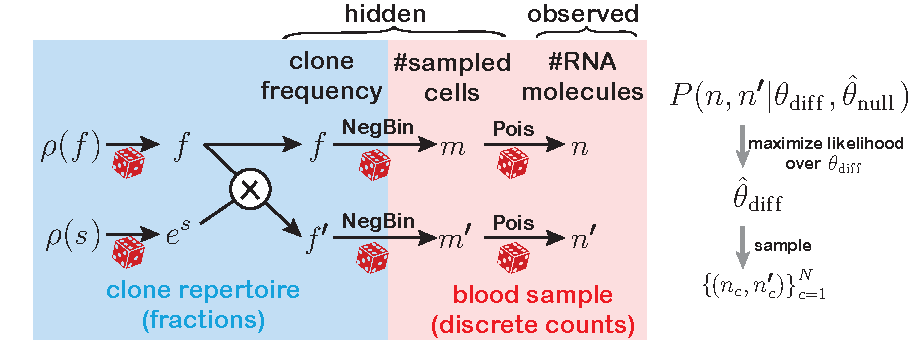
\includegraphics{fig2_diffexprmodel_schematic}
\centering{}
\caption{
\emph{Differential expression model structure and learning procedure}. $P(n|f)$ is set as a negative binomial distribution in cell counts controlling the scale parameter of a Poisson distribution of molecule counts. In the differentially expressed condition (prime-decorated quantities), the parameters, $\theta_{diff}$, of the prior distribution, $\rho(c)$, of fold-change, $c$, are learned by maximizing the marginal likelihood (see section \textit{Fold change prior}) with respect to $\theta_{diff}$, keeping the remaining parameters, $\theta_{null}$, fixed to their ML estimates, $\hat{\theta}_{null}$, previously obtained using same-day replicate data (see fig. \ref{fig:nullstats}). 
\label{fig:modelstruct}}
\end{figure*}

% \begin{figure*}[ht!]
% \includegraphics[width=\textwidth]{fig2_learnednullparas}
% \centering{}
% \caption{
% \emph{Histograms of learned null model parameters}. The clone frequency distribution $\rho(f)=\int_{f_{min}}^{1}f^\alpha\textrm{d}f/Z$, is determined by the power $\alpha$ and minimal frequency, $f_{min}$. The cell count variance, $\sigma^2_m=fM+a(fM)^\gamma$, is determined by the total number of cells in the sample, $M$, and the power, $\gamma$, and coefficient, $a$, controlling the over-dispersion.{\color{red}update figure with remaining data}
% \label{fig:nullparas}}
% \end{figure*}

\begin{figure}[ht!]
%\includegraphics[width=\linewidth]{fig2_learnednullparas}
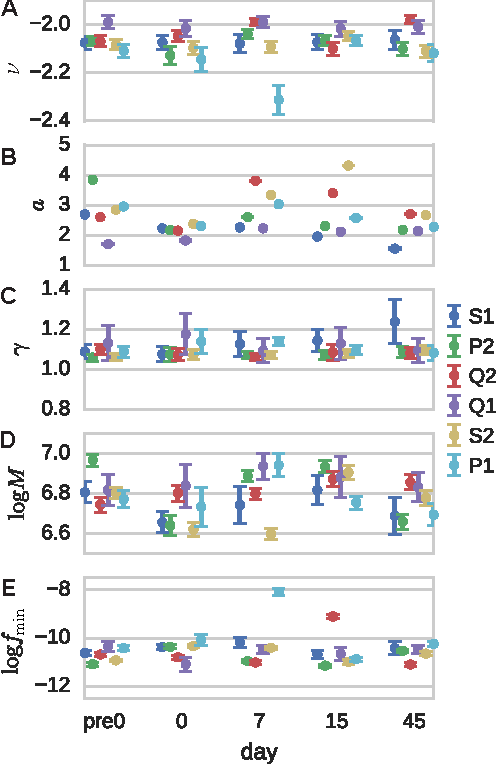
\includegraphics{fig3_learnednullparas}
\centering{}
\caption{
\emph{Learned null model parameters}. Shown is the same data from fig. \ref{fig:nullparas}, plotted separately for each donor and time point. Error bars are the inverse standard deviation of a Gaussian approximation around the maximum of the likelihood, i.e. the Cramer-Rao lower bound of the variance of the estimator. 
\label{fig:nullparas_timeseries}}
\end{figure}

  

\begin{figure}[ht!]
%\includegraphics[width=\linewidth]{fig2_learnednullparas}
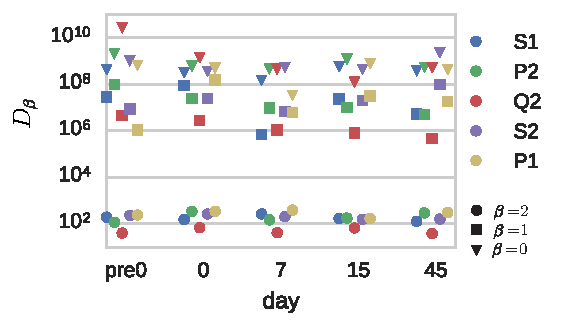
\includegraphics{fig4_div_estimates}
\centering{}
\caption{
\emph{Diversity estimates.} Shown are diversity estimates obtained from the Renyi entropies, $H_\beta$, of the inferred clone frequency distributions for $\beta=1$ (Shannon entropy) and $\beta=2$ (Simpson index), across donors and days.
\label{fig:div_estimates}}
\end{figure}

% \begin{figure}[ht!]
% 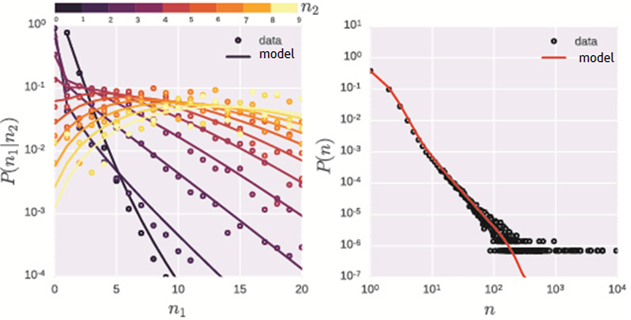
\includegraphics[width=\linewidth]{conditional_marginal}
% \centering{}
% \caption{
% \emph{Null model marginals and conditionals}. The marginal, $P(n_1|\theta_n)=\sum_{n_2}P(n_1,n_2|\theta_n)$ (a), and conditional $P(n_1|n_2\theta_n)=P(n_1,n_2|\theta_n)/P(n_1|\theta_n)$ (b), distributions.{\color{red} Add variance to this. Maybe also likelihood surface. update figure with new data}
% \label{fig:modelfit}}
% \end{figure}

% \begin{itemize}
% 	\item  presentation question: do we start with data description and plot first (See figure above) or immediately develop model first and only show data when showing fit?
% \end{itemize}

% \begin{table*}%[H] add [H] placement to break table across pages
% \caption{Null Model Selection. Akaike Information Criterion (AIC) and Bayesian Information Criterion (BIC) for the for null models tested. Shown here are averages and standard deviations over 6 donors (n.b. donor-specific parameters are used throughout). \label{Tbl1:NullModelCompare}}
% \begin{ruledtabular}
% \begin{tabular}{c|c|c|c|c|c|c|c}
% index	& label					&parameters					& day pre0 (A/BIC)& day 0 (A/BIC) 	&day 7 (A/BIC) 	&day 15 (A/BIC) 	&day 45 (A/BIC)    	\\
% \hline
% 1 		& $\mathrm{Poisson}$ 	 			&$\gamma$,$f_{\textrm{min}}$				& 7.02e6/7.02e6				& x/x					& x/x  				& x/x  				& x/x\\
% 2 		& $\mathrm{NegBin}$				 	&$\gamma$,$a_n$,$\delta_n$,$f_{\textrm{min}}$  				& 5.854e6/5.854e6					& x/x				& x/x  				& x/x  				& x/x\\
% 3 		& $\mathrm{Poisson}\rightarrow \mathrm{NegBin}$ 	&$\gamma$,$M$,$a_n$,$\delta_n$,$f_{\textrm{min}}$	& 5.841e6/5.841e6					& x/x 				& x/x  				& x/x  				& x/x\\ 
% 4 		& $\mathrm{NegBin}\rightarrow \mathrm{Poisson}$  &$\gamma$,$M$,$a_m$,$\delta_m$,$f_{\textrm{min}}$ 		& 5.839e6/5.839e6					& x/x 				& x/x  				& x/x  				& x/x\\ 
% 
% \end{tabular}
% \end{ruledtabular}
% \end{table*}



% \begin{figure}[h!]
% %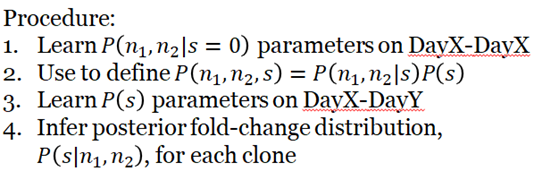
\includegraphics{procedure.png}
% \caption{
% \emph{Supp. Fig: Self-consistent reinference of null model}.
% \label{fig:suppfig2_reinf_null}}
% \end{figure}

% \begin{figure}[h!]
% %\includegraphics{suppfig1_null_model_example}
% \caption{
% \emph{Supp. Fig: Failure with Poisson model}.
% \label{fig:suppfig1_Poisfail}}
% \end{figure}

% \begin{figure}[h!]
% 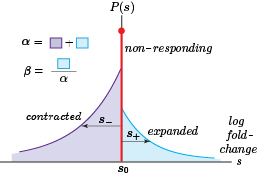
\includegraphics{schematic}
% \centering{}
% \caption{
% \emph{Functional forms of prior on clone size log fold-change}. $P(s)$, eq. \ref{eq:genPs}, is parametrized most generally here by an effect size for both expansion, $s_+$, and contraction,$s_-$, with an expanded fraction, $\beta$ of changed clones, the latter fraction of which itself a parameter, $\alpha$. Expansion and contraction is relative to the functions center, $s_0$, which can be fixed by the constraint $\langle f_1 \rangle=\langle f_2 \rangle$.
% \label{fig:Ps}}
% \end{figure}


% \begin{figure}[ht!]
% %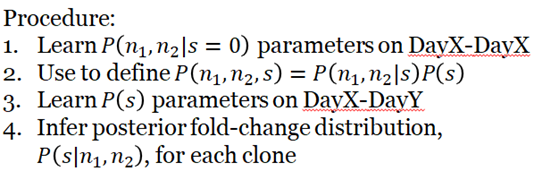
\includegraphics{procedure.png}
% %centering{}
% \caption{
% \emph{Supp. Fig: Self-consistent reinference of diffexpr model}.
% \label{fig:suppfig2_reinf_diffexpr}}
% \end{figure}

% \begin{figure}[ht!]
% %\includegraphics{fig2_null_model_example}
% %\centering{}
% \caption{
% \emph{Analysis of sloppiness of model: description of max-Likelihood manifold and possibly reduced description}
% \label{fig:Data}}
% \end{figure}
% 
% \begin{figure}[ht!]
% %\includegraphics{fig2_null_model_example}
% %\centering{}
% \caption{
% \emph{Evolution of parameters}. 
% \label{fig:timeevo}}
% \end{figure}



% (old) Text:
% 
% Armed with a well fit model of the same day variation, we generalized the model to apply to different days using a log fold change variable sampled from some distribution that controls the expansion or contraction that the second clone exhibits. 
% And, marginalizing out the hidden fold change variable, we again obtain a joint count distribution that we can use to fit the parameters of rho(s) to maximize the likelihood of the data. 
% We choose to restrict rho(s) to a two-parameter family of symmetric functions, with a parameter alpha the fraction of the repertoire that responds, and the sbar a typical effect size that controls the mean of a symmetric exponential function around 0 log fold change where the rest of clones are left as a delta function component.
% Doing the inference on alpha and sbar, and using the day 0 as the reference, we saw how the fraction of the perturbed repertoire rises and falls around day 15, as expected. 
 
% \begin{figure}[ht!]
% %\includegraphics{fig2_null_model_example}
% %\centering{}
% \caption{
% \emph{Posteriors}. Some example posteriors. Distributions of slow, smed, shigh, and Pval. Volcano plot.
% \label{fig:posteriors}}
% \end{figure}


% Old Text from presentation:
% 
% To do that we look at the posterior probability of a clone being expanded or contracted for a given count pair, where here we plot it as a confidence and versus the pair’s expected fold change that comes out the model, a volcano plot, commonly used in RNAseq.
% We set a threshold on confidence and all pairs above this threshold are candidates for being selective to the vaccine. 
% Take a look at the two sets of points associated with the first count being 0 and 1, and with the second count of the data points increases with the expected fold change. 
% Remember that low counts convey little frequency and thus expansion information: the initial frequency could have been anything small and so we have to go to pretty high fold change, i.e. high n2, before we can say that this expansion is significant. 
% In particular, if we condition instead on the first count being 1, the expansion becomes significant at lower fold change, as the first count more reliably conveys information about it’s frequency. and so on with increasing count, and similarly for contraction.
% These are candidate clones ‘specific to the vaccines’. But how do we do we know that this is in fact the case.
% Experimental work performed a functional test by adding a gate for IFN gamma and sequenced this IFN enriched pool indeed show the vast majority show a strong functional response, validating our method. 

% \begin{figure}[ht!]
% 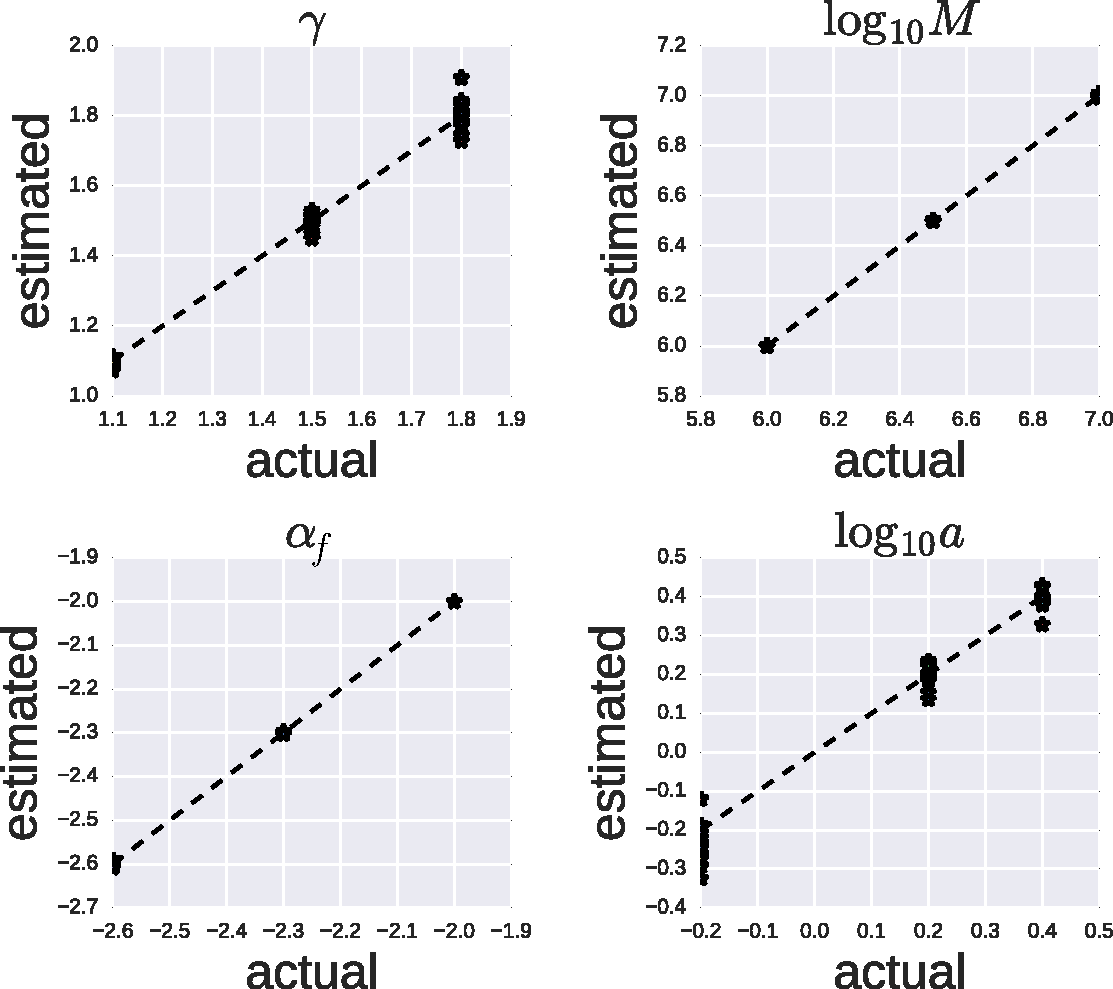
\includegraphics[width=\linewidth]{NB_Pois_nullpara_fits}
% \centering{}
% \caption{
% \emph{Reinferring null model parameters}. Shown are the actual and estimated values of the null model parameters used to validate the null model inference procedure over the range exhibited by the data. A 3x3x3x3 grid of points were sampled and results collapsed over each parameter axis. $f_{min}$ was fixed to satisfy the normalization constraint. {\color{red} Add $f_{min}$ dependence and realign into 2x2 subfigure grid}
% \label{fig:reinfer_null}}
% \end{figure}


%\bibliography{references}

\end{document}  












